% Study deck for the Dec 2 presentation. Build: tectonic study_deck.tex
% Style rule: no em dashes.
\documentclass[aspectratio=169,10pt]{beamer}
\usepackage{tikz,booktabs,amsmath,xcolor}
\usetikzlibrary{positioning,arrows.meta,calc}

\definecolor{ink}{HTML}{1F2430}
\definecolor{accent}{HTML}{2F6FDE}
\definecolor{warm}{HTML}{D9622B}
\definecolor{good}{HTML}{2E8B57}
\definecolor{soft}{HTML}{EEF2FA}
\definecolor{mute}{HTML}{6B7280}
\setbeamercolor{normal text}{fg=ink,bg=white}
\setbeamercolor{frametitle}{fg=accent}
\setbeamercolor{structure}{fg=accent}
\setbeamercolor{alerted text}{fg=warm}
\setbeamerfont{frametitle}{series=\bfseries,size=\Large}
\setbeamertemplate{navigation symbols}{}
\setbeamertemplate{itemize items}{\textcolor{accent}{\raisebox{0.1ex}{$\bullet$}}}
\setbeamertemplate{footline}{\hfill\textcolor{mute}{\scriptsize\insertsection\quad\insertframenumber/\inserttotalframenumber}\hspace{1em}\vspace{0.6em}}
\setbeamertemplate{section page}{\centering\vfill{\color{accent}\Huge\bfseries\insertsection}\vfill}
\AtBeginSection{\begin{frame}[plain]\sectionpage\end{frame}}

% "Say it" box: what to tell the audience on this slide
\newcommand{\say}[1]{\par\vfill\noindent\colorbox{soft}{\parbox{\dimexpr\textwidth-2\fboxsep\relax}{\small\textbf{\textcolor{accent}{Say it:}} #1}}}
\newcommand{\qa}[2]{\textbf{\textcolor{accent}{Q.}} \textbf{#1}\\[0.2em]{\small #2}\par\medskip}

\title{Launch-Bound and Cache-Aware}
\subtitle{Predicting VLA inference latency and CUDA-graph speedup across GPU generations\\[0.4em]
\small Study deck for the December 2 presentation}
\author{Aditya Maddur Guruprakash \and Archana Jayakumar \and Shrikar Madhu}
\institute{NYU, GPU Architecture and Programming, Fall 2026, Project 2 (flavor B)}
\date{}

\begin{document}

\begin{frame}[plain]\titlepage\end{frame}

\begin{frame}{How to use this deck}
\begin{itemize}
\item Five parts: \textbf{the problem}, \textbf{what we measured}, \textbf{the model},
  \textbf{extensions by the team}, \textbf{takeaways}. Then a \textbf{numbers cheat sheet} and
  \textbf{Q\&A practice} (26 questions with answers).
\item Every slide has a \colorbox{soft}{\small\textbf{\textcolor{accent}{Say it:}}} box: the one or
  two sentences you would actually say out loud.
\item All numbers come from the report (\texttt{paper/main.pdf}) and \texttt{results/*.md}.
\end{itemize}
\vspace{1em}
\textbf{The whole project in one sentence:}
\begin{center}\begin{minipage}{0.85\textwidth}\centering\large
Small robot policies on a GPU are slow because of \alert{thousands of tiny kernel launches},
not because the GPU lacks FLOPs or bandwidth; so predicting their speed on another GPU, and
what CUDA graphs will buy, needs a model of \alert{launch and per-kernel latency}.
\end{minipage}\end{center}
\end{frame}

% ------------------------------------------------------------------
\section{1. The problem}

\begin{frame}{What is a VLA policy?}
\begin{columns}[T]
\column{0.55\textwidth}
\begin{itemize}
\item \textbf{Vision-Language-Action} model: camera images + a text instruction in, robot
  actions out.
\item Two halves:
  \begin{itemize}
  \item \textbf{Prefix}: vision encoder + language model read the images once and fill a
    KV cache.
  \item \textbf{Action expert}: a small transformer that turns noise into an \emph{action
    chunk} (50 future actions) in 10 \textbf{flow-matching} (denoising) steps.
  \end{itemize}
\item Runs at \textbf{batch 1}: one robot, one observation, as fast as possible.
\item Main workload: \textbf{SmolVLA} (450M parameters, FP16).
\end{itemize}
\column{0.43\textwidth}
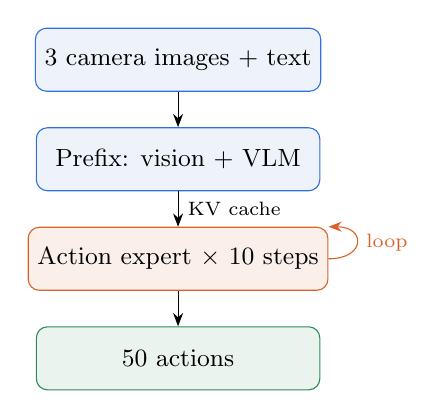
\begin{tikzpicture}[node distance=0.45cm, every node/.style={font=\small}]
\node[draw=accent,fill=soft,rounded corners,minimum width=3.6cm,minimum height=0.8cm] (img) {3 camera images + text};
\node[draw=accent,fill=soft,rounded corners,minimum width=3.6cm,minimum height=0.8cm,below=of img] (pre) {Prefix: vision + VLM};
\node[draw=warm,fill=warm!10,rounded corners,minimum width=3.6cm,minimum height=0.8cm,below=of pre] (exp) {Action expert $\times$ 10 steps};
\node[draw=good,fill=good!10,rounded corners,minimum width=3.6cm,minimum height=0.8cm,below=of exp] (act) {50 actions};
\draw[-{Stealth}] (img)--(pre); \draw[-{Stealth}] (pre)--node[right]{\scriptsize KV cache} (exp); \draw[-{Stealth}] (exp)--(act);
\draw[-{Stealth},warm] (exp.east) to[out=0,in=0,looseness=3] node[right]{\scriptsize loop} (exp.north east);
\end{tikzpicture}
\end{columns}
\say{A VLA reads the cameras once, then runs a small network ten times to produce the next
second of robot motion. That ten-step loop is where most of the kernels are.}
\end{frame}

\begin{frame}{Why batch-1 inference is a strange GPU workload}
\begin{columns}[T]
\column{0.5\textwidth}
SmolVLA, one step on an A100:
\begin{itemize}
\item \textbf{13,190 kernels} per step
\item median kernel: \textbf{3.3\,$\mu$s}; 78\% under 5\,$\mu$s
\item eager step 377\,ms, but GPU busy only \textbf{58\,ms (15\%)}
\item median achieved occupancy 13.5\% (ncu, 2080 Ti)
\end{itemize}
\column{0.48\textwidth}
Classic GPU performance models (Hong and Kim, GPUPerf, rooflines) assume kernels that
\emph{fill} the GPU and run for milliseconds.\\[0.6em]
Here the GPU is mostly \alert{idle, waiting for the CPU} to tell it what to do next.
\end{columns}
\say{The GPU is busy only 15\% of the time. The other 85\% it waits for Python and PyTorch on
the CPU to launch the next tiny kernel. That is the regime classic models do not cover.}
\end{frame}

\begin{frame}{Eager launches vs CUDA graphs (the key intuition)}
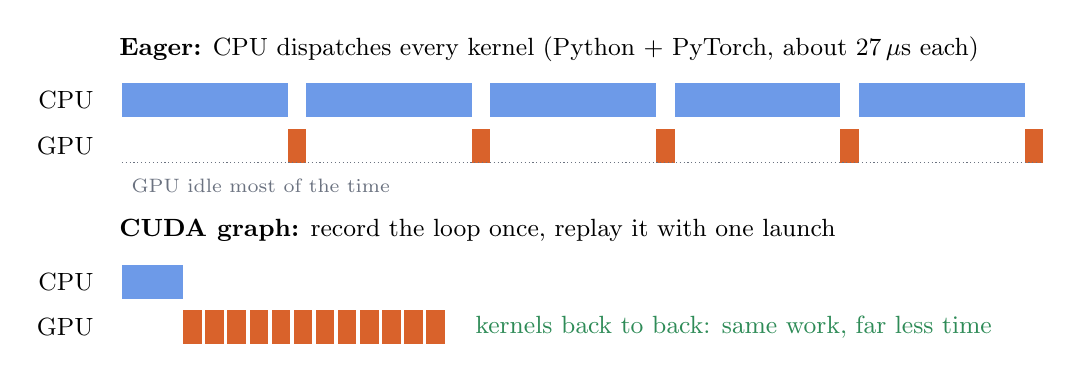
\begin{tikzpicture}[x=0.78cm,y=0.72cm,font=\small]
\node[anchor=west] at (-0.2,4.3) {\textbf{Eager:} CPU dispatches every kernel (Python + PyTorch, about 27\,$\mu$s each)};
\node[anchor=east] at (-0.3,3.4) {CPU}; \node[anchor=east] at (-0.3,2.6) {GPU};
\foreach \i in {0,...,4} {
  \fill[accent!70] (\i*3,3.1) rectangle ++(2.7,0.6);
  \fill[warm] (\i*3+2.7,2.3) rectangle ++(0.3,0.6);
}
\draw[mute,densely dotted] (0,2.3)--(15,2.3);
\node[anchor=west,mute] at (0,1.9) {\scriptsize GPU idle most of the time};
\node[anchor=west] at (-0.2,1.1) {\textbf{CUDA graph:} record the loop once, replay it with one launch};
\node[anchor=east] at (-0.3,0.2) {CPU}; \node[anchor=east] at (-0.3,-0.6) {GPU};
\fill[accent!70] (0,-0.1) rectangle ++(1.0,0.6);
\foreach \i in {0,...,11} { \fill[warm] (1.0+\i*0.36,-0.9) rectangle ++(0.3,0.6); }
\node[anchor=west,good] at (5.6,-0.6) {kernels back to back: same work, far less time};
\end{tikzpicture}
\begin{itemize}
\item A graph removes the per-kernel CPU cost, but needs \textbf{static shapes and no host
  syncs}: we could graph SmolVLA's loop, not its vision encoder (a data-dependent
  \texttt{arange}).
\item \textbf{Hybrid} step = eager prefix + graphed loop (what you would deploy).
\end{itemize}
\say{Eager mode is like ordering items one at a time; a CUDA graph hands over the whole
shopping list at once. Same kernels, but the GPU no longer waits for the CPU.}
\end{frame}

\begin{frame}{How big is the effect? (SmolVLA on the A100)}
\centering
\begin{tabular}{lrr}\toprule
 & eager & with CUDA graph\\\midrule
10-step denoising loop & 316\,ms & \textbf{35.8\,ms} (8.8$\times$)\\
full step (hybrid) & 377\,ms & \textbf{94\,ms} (4.0$\times$)\\\bottomrule
\end{tabular}
\vspace{1em}
\begin{itemize}
\item Our \textbf{C++ replay} of the same kernels runs the loop eager in 44.7\,ms vs 407\,ms in
  PyTorch (2080 Ti): about \textbf{89\% of eager time is framework dispatch}.
\item Loop graph speedup ranges from \textbf{4.6$\times$ to 22.5$\times$} across our four GPUs.
  Why it varies so much is a central question.
\item Outputs are \textbf{bit-exact}: graph vs eager max $|$diff$|$ = 0 in every run.
\end{itemize}
\say{Graphs make the loop almost nine times faster on the A100, and the same code in C++ shows
that nearly 90\% of eager time is Python and PyTorch overhead, not GPU work.}
\end{frame}

\begin{frame}{The question we answer (Project 2, flavor B)}
\begin{block}{Flavor B}
Knowing the performance of a kernel (here: a whole policy step) on one GPU, can we predict
it on another GPU with different specifications?
\end{block}
We predict on a \textbf{target} GPU, from a trace on a \textbf{source} GPU:
\begin{enumerate}
\item the eager step latency,
\item the graphed loop latency,
\item the hybrid step latency,
\item the CUDA-graph speedup (and whether to bother capturing).
\end{enumerate}
\textbf{Motivation from public benchmarks (Yotta Labs, Aug 2026):} H200 \emph{slower} than H100
on OpenVLA (273 vs 173\,ms) and GR00T (297 vs 180\,ms); OpenVLA stuck near 173\,ms on H100 and
PRO 6000. Spec sheets cannot explain this.
\say{The H200 has more bandwidth than the H100 and is still slower on OpenVLA. If spec ratios
cannot explain that, we need a model built around what actually limits these workloads.}
\end{frame}

% ------------------------------------------------------------------
\section{2. What we measured}

\begin{frame}{Hardware: four GPU generations, four very different hosts}
\centering\small
\resizebox{\textwidth}{!}{\begin{tabular}{llrrrl}\toprule
GPU & arch & SMs & L2 & DRAM BW (measured) & host CPU\\\midrule
RTX 2080 Ti (cuda2, \textbf{source}) & Turing & 68 & 5.5\,MB & 582\,GB/s & Xeon E5-2660 v3\\
TITAN V (cuda3) & Volta & 80 & 4.5\,MB & 648\,GB/s & Xeon Gold 5118\\
RTX 4070 (cuda5) & Ada & 46 & 36\,MB & 475\,GB/s & Xeon E5-2650 v2 (2013)\\
A100-SXM4-40GB (NYU HPC) & Ampere & 108 & 40\,MB & 1479\,GB/s & cloud Xeon 2.2\,GHz\\\bottomrule
\end{tabular}}
\vspace{0.8em}
\begin{itemize}
\item Also used: GTX TITAN X (cuda4, C++ calibration only), a 2$\times$A100 node (placement),
  an RTX PRO 6000 Blackwell on Empire AI (multi-policy).
\item The L4 partition never booted (dropped); our account could not use T4/V100/H100.
\item Note the hosts: the \textbf{host CPU matters as much as the GPU} here.
\end{itemize}
\say{We cover Turing, Volta, Ada and Ampere, and the CPUs behind them range from a 2013 Xeon to
a cloud server. That spread turns out to be essential.}
\end{frame}

\begin{frame}{Workloads: seven policies, three regimes}
\small
\begin{tabular}{llll}\toprule
Policy & size / precision & what we graph & regime\\\midrule
SmolVLA & 450M, FP16 & 10-step flow loop & \textbf{dispatch bound}\\
$\pi_0$, $\pi_{0.5}$ & PaliGemma-based, FP16 & 10-step flow loop & dispatch bound\\
$\pi_0$-FAST & autoregressive, 256 tokens & decode loop & dispatch + bandwidth\\
OpenVLA-7B & 7B, FP16 (A100 only) & 6 decode steps & 4$\times$ dispatch bound decode\\
ACT & 52M, FP32 & whole step & \textbf{mixed} (2.4$\times$)\\
Diffusion Policy & 263M, FP32 & 100-step DDPM loop & \textbf{GPU bound} (1.0$\times$)\\\bottomrule
\end{tabular}
\vspace{0.6em}
\begin{itemize}
\item Sweeps (SmolVLA): 1 to 3 cameras, 5/10/20 flow steps, chunk 25/50/100, batch 1 to 16.
\item FP16 on Turing/Volta (no BF16): checked activations stay in FP16 range for $\pi_0$ and
  $\pi_{0.5}$; $\pi_0$-FAST overflows in FP16, so its FP16 runs are timing only.
\end{itemize}
\say{The policies span the range from almost pure launch overhead (SmolVLA) to fully GPU bound
(Diffusion Policy), which lets us test where the model holds and where it breaks.}
\end{frame}

\begin{frame}{How we measured (and why you can trust the numbers)}
\begin{columns}[T]
\column{0.5\textwidth}
\textbf{Timing discipline}
\begin{itemize}\small
\item warm-up, \texttt{CUDA\_MODULE\_LOADING=EAGER}
\item CUDA events / host timers after sync
\item medians of $\geq$ 20 repetitions
\item idle-GPU check before every stage (CIMS is shared)
\item eager timings pinned to the GPU's NUMA node
\item same PyTorch build (2.10 / CUDA 12.8) on every host
\end{itemize}
\column{0.48\textwidth}
\textbf{Tools}
\begin{itemize}\small
\item PyTorch profiler (CUPTI) for kernel traces
\item Nsight Compute: DRAM/L2 bytes, occupancy
\item Nsight Systems: timeline figure
\item our CUDA C++ microbenchmarks and C++ replay
\end{itemize}
\textbf{Sanity checks}
\begin{itemize}\small
\item graph vs eager outputs bit-exact
\item repeat runs within 1 to 2\%
\item fresh-clone rebuild on cuda2 passes
\end{itemize}
\end{columns}
\say{We were strict about timing because the effects we model are microseconds per kernel:
warm-up, idle GPUs, pinned CPUs, repeated runs and bit-exact outputs.}
\end{frame}

\begin{frame}{Our CUDA C++ code (the course requirement)}
\begin{itemize}
\item \textbf{Calibration microbenchmarks} (\texttt{bench/calib}):
  \begin{itemize}\small
  \item launch latency: empty kernel eager 2.5\,$\mu$s apart, graph node 0.8\,$\mu$s (A100)
  \item spin-kernel chains: eager costs about \textbf{2\,$\mu$s extra per kernel even for
    long kernels}, a GPU-side cost, not CPU starvation
  \item bandwidth / L2 sweep: finds the effective L2 (A100: 20 to 27\,MB of 40)
  \end{itemize}
\item \textbf{Our own kernels} (\texttt{bench/kernels}): WMMA FP16 GEMM with split-K, FP32 GEMM,
  online-softmax attention, LayerNorm/RMSNorm, RoPE, SiLU/GELU. All pass correctness checks
  vs cuBLAS / CPU.
\item \textbf{C++ replay} of the traced SmolVLA step (\texttt{bench/chains}): the real kernel
  list, eager vs graph. 10-step loop as a graph: 39.4\,ms vs 40.1\,ms real PyTorch graph.
\end{itemize}
\say{Everything builds with nvcc 12.4 on the CIMS machines. The C++ replay is our proof that
the eager slowness is software, because the same kernels launched from C++ are fast.}
\end{frame}

\begin{frame}{Finding 1: small kernels are latency bound}
\begin{itemize}
\item Identical PyTorch kernels under 6\,$\mu$s take the \textbf{same time} on the A100 and the
  2080 Ti (ratio 0.98 to 1.02), despite 2.5$\times$ the bandwidth.
\item Graphed loop: A100 35.6\,ms vs 2080 Ti 39.8\,ms, only \textbf{11\% faster}.
\item Real ``graph slot'' per kernel (duration + node gap): A100 3.0, 2080 Ti 3.4, TITAN V
  5.2\,$\mu$s.
\item \textbf{Why is the TITAN V slow?} Its \emph{sustained} clock: 1335\,MHz under load vs
  1950\,MHz on the 2080 Ti. Ratio 1.46 matches the per-kernel ratio 1.54.
\item Clock alone does not cross architectures: the A100 runs at 1410\,MHz yet is as fast as
  the 2080 Ti per small kernel.
\end{itemize}
\say{For tiny kernels bandwidth does not matter; start-up latency and the clock the GPU really
runs at do. That is why spec-sheet scaling fails.}
\end{frame}

\begin{frame}{Finding 2: the GPU ordering inverts between eager and graph}
\centering
\begin{tabular}{lrrr}\toprule
GPU (host) & eager step & graphed loop & loop speedup\\\midrule
TITAN V (fast host) & \textbf{341\,ms} (fastest) & 61.4\,ms (slowest) & 4.6$\times$\\
A100 & 383\,ms & 35.6\,ms & 9.0$\times$\\
RTX 2080 Ti & 484\,ms & 39.8\,ms & 10.2$\times$\\
RTX 4070 (2013 host) & 607\,ms (slowest) & \textbf{22.8\,ms} (fastest) & \textbf{22.5$\times$}\\\bottomrule
\end{tabular}
\vspace{0.8em}
\begin{itemize}
\item Eager speed is set by the \textbf{host CPU}; graph speed by the \textbf{GPU}.
\item So the graph speedup is a property of the \textbf{host-GPU pair}, not the workload alone.
\item Same inversion for ACT, $\pi_0$, $\pi_{0.5}$. Our model predicts it from every source GPU;
  bandwidth scaling never does.
\end{itemize}
\say{The slowest GPU in eager mode is the fastest with graphs. Graphs shift the bottleneck from
the CPU to the GPU, so the GPU ranking flips.}
\end{frame}

\begin{frame}{Finding 3: the L2 cache is second order (for these policies)}
\begin{itemize}
\item Hypothesis (in our title): if a step's weights fit in L2, small kernels get faster.
\item Test: C++ replay with all weights in a pool of $N$ MB, sweep $N$ = 3 to 256\,MB.
\item Result: weights in L2 vs streamed from DRAM saves only \textbf{1 to 13\%}
  (A100 cuBLAS 31.2 vs 32.2\,ms). Knee sits at each GPU's L2 size.
\item Why: each denoising step streams \textbf{250\,MB of weights}: 1.7\,ms of DRAM time in a
  32\,ms loop. The rest is per-kernel latency.
\item The real expert's weights exceed every L2 we had (max 40\,MB).
\item When would it matter? A small policy on a huge L2: ACT (about 104\,MB in FP16) on an RTX
  PRO 6000 (128\,MB L2). We describe that experiment; it is future work.
\end{itemize}
\say{We tested the cache half of our hypothesis and it came out small: the weights are bigger
than any L2 we could measure, so latency dominates. We are explicit about when it would matter.}
\end{frame}

% ------------------------------------------------------------------
\section{3. The model}

\begin{frame}{Idea: replay the step on two timelines}
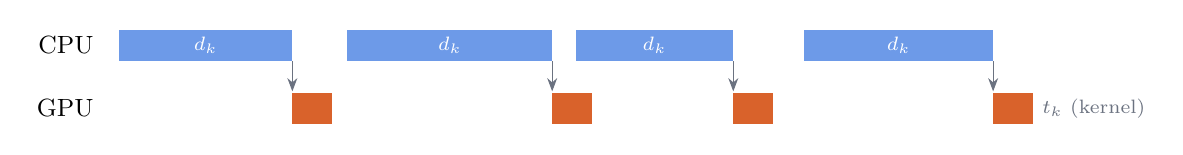
\begin{tikzpicture}[x=1cm,y=0.8cm,font=\small]
\node[anchor=east] at (-0.2,1) {CPU}; \node[anchor=east] at (-0.2,0) {GPU};
\foreach \i/\w in {0/2.2,1/2.6,2/2.0,3/2.4} {
  \pgfmathsetmacro{\x}{\i*2.9}
  \fill[accent!70] (\x,0.75) rectangle ++(\w,0.5);
  \node[font=\scriptsize,white] at (\x+\w/2,1) {$d_k$};
  \fill[warm] (\x+\w,-0.25) rectangle ++(0.5,0.5);
  \draw[-{Stealth},mute] (\x+\w,0.75)--(\x+\w,0.27);
}
\node[anchor=west,font=\scriptsize,mute] at (11.6,0) {$t_k$ (kernel)};
\end{tikzpicture}
\vspace{0.4em}
\begin{itemize}
\item \textbf{CPU} spends $d_k = c_{\mathrm{op}(k)} + p$ on kernel $k$:\\
  $c$ = PyTorch dispatch cost of that op type (measured table: add 7\,$\mu$s, linear 17 to
  22\,$\mu$s, SDPA 31\,$\mu$s), $p$ = Python time per kernel (fitted).
\item \textbf{GPU} starts kernel $k$ at $\max(\text{CPU ready},\ \text{previous kernel done} + g_{\mathrm{eager}})$,
  runs it for $t_k$. Host copies synchronize the two timelines.
\item \textbf{Graph mode}: $T_{\mathrm{graph}} = L_{\mathrm{graph}} + \sum_k (t_k + \delta_{\mathrm{node}})$.
\end{itemize}
\say{We simulate the CPU and the GPU side by side. Whichever is slower at each kernel sets the
pace; in eager mode that is almost always the CPU.}
\end{frame}

\begin{frame}{Two fitted numbers, both on the source only}
\begin{columns}[T]
\column{0.5\textwidth}
\textbf{$b$: profiler bias}
\begin{itemize}\small
\item Tracing adds about \textbf{1\,$\mu$s per kernel} (11.3\,ms per graph replay on every GPU).
\item That is a third of a 3\,$\mu$s kernel, so we subtract it before summing.
\item Fitted once per source machine.
\end{itemize}
\column{0.48\textwidth}
\textbf{$p$: Python time per kernel}
\begin{itemize}\small
\item Time between aten ops: Python modules, HF code.
\item About 17\,$\mu$s on the A100 host.
\item \textbf{A host property}: 2080 Ti host 20.5 to 23.1\,$\mu$s and TITAN V host 12.7 to
  13.8\,$\mu$s, across SmolVLA, $\pi_0$, $\pi_{0.5}$, $\pi_0$-FAST.
\end{itemize}
\end{columns}
\vspace{0.8em}
Fitted on \textbf{one} baseline run, then held fixed for all other configurations and all
targets. Same-GPU held-out error: SmolVLA eager 1.3 to 4.5\%, graph loop 0.2 to 1.7\%.
\say{Only two numbers are fitted, and only on the source. Everything about the target comes
from cheap microbenchmarks run on the target.}
\end{frame}

\begin{frame}{Moving kernels to another GPU: graph slots}
\begin{itemize}
\item Do not scale raw durations by bandwidth or FLOPs. Instead transfer each kernel's
  \textbf{slot} $u_k = t_k + \delta$ (what it really costs inside a graph).
\item Ratio per \textbf{op class} (elementwise, allocating op, GEMM, attention, conv), measured
  by tiny PyTorch microbenchmarks replayed as CUDA graphs on source and target:
  \[u_k^T = r_c \min(u_k, \tau_c) + r_{\mathrm{bw}} \max(u_k - \tau_c, 0)\]
  (the bandwidth tail only for long kernels).
\item This captures architecture \emph{and} sustained clock in one measured number.
\end{itemize}
\textbf{Host side (final variant \texttt{slot\_drv})}
\begin{itemize}
\item Dispatch costs from the target's own table.
\item $p$ scaled by the ratio of the dispatch tables \emph{after} subtracting each host's bare
  \texttt{cudaLaunchKernel} cost: the framework part, not the driver part.
\end{itemize}
\say{We ask the target GPU how long a small op of each kind takes in a graph, and scale every
traced kernel of that kind by that ratio.}
\end{frame}

\begin{frame}{Results: cross-GPU accuracy (MAPE, source $\neq$ target)}
\centering\small
\begin{tabular}{lrrrr}\toprule
Workload (GPUs) & eager & graph loop & hybrid & loop speedup\\\midrule
SmolVLA (4) & 20.2 & \textbf{15.3} & 13.0 & 22.0\\
SmolVLA (3 comparable hosts) & \textbf{6.6} & 16.2 & \textbf{5.5} & 21.7\\
$\pi_0$ (3) & 17.8 & 12.8 & 11.2 & 31.0\\
$\pi_{0.5}$ (3) & 11.9 & 10.4 & 17.8 & 30.8\\
$\pi_0$-FAST (3) & 19.2 & 9.3 & 7.1 & 13.1\\
ACT (4) & 28.0 & 12.2 & & 21.2\\
Diffusion, default cuDNN (4) & 39.8 & 41.9 & 41.3 & 3.6\\\midrule
SmolVLA, spec bandwidth scaling & 25.5 & \alert{96.4} & 44.6 & 64.0\\\bottomrule
\end{tabular}
\vspace{0.5em}
\begin{itemize}\small
\item Exact ranking of the four GPUs: \textbf{65\%} of cases vs 26\% for bandwidth scaling.
\end{itemize}
\say{The graphed loop transfers within 9 to 16\% for every dispatch-bound policy, where
bandwidth scaling is off by almost 100\%. Eager is good between similar hosts and worse into
the old host.}
\end{frame}

\begin{frame}{Against the baselines}
\begin{columns}[T]
\column{0.5\textwidth}
\textbf{VLA-Perf} (NVIDIA, 2026): spec-sheet roofline per operator, explicitly no launch or
runtime overhead. We ran their code on our models:
\begin{itemize}\small
\item SmolVLA on A100: predicts \textbf{3.9\,ms} vs 383 eager / 95 hybrid / 35.6 graph loop
\item MAPE 86 to 98\% on every quantity
\item graph speedup is 1.0$\times$ by construction
\end{itemize}
Not wrong arithmetic: it is an \emph{upper bound}. The gap to reality is launch and
per-kernel latency.
\column{0.48\textwidth}
\textbf{Ablation: how much target calibration?}
\begin{itemize}\small
\item spec only: eager 34\%, graph loop 38\%, ranking 20\%
\item + C++ microbenchmarks: barely helps
\item + PyTorch dispatch table: ranking 57\%
\item + graph-slot table: graph loop 31 $\rightarrow$ 15\%
\end{itemize}
A few minutes of PyTorch microbenchmarks on the target are what make transfer work.
\end{columns}
\say{The best roofline model is two orders of magnitude optimistic here. The cheap PyTorch
microbenchmarks on the target are the ingredient that matters.}
\end{frame}

\begin{frame}{Where the model breaks (and what that teaches)}
\begin{enumerate}
\item \textbf{A very different host CPU} (RTX 4070 on the 2013 Xeon):
  \begin{itemize}\small
  \item its launch call costs 8.7\,$\mu$s (others 1.9 to 2.6); microbenchmarks say 2.3 to
    2.5$\times$ slower, the real eager step is only 1.6 to 1.8$\times$ slower
  \item eager predictions into/out of it 20 to 44\% off; the graph loop still 9 to 10\%
  \item no single CPU index fits all hosts: open problem
  \end{itemize}
\item \textbf{The library changes the algorithm} (Diffusion Policy, cuDNN default heuristic):
  \begin{itemize}\small
  \item a different conv algorithm on each architecture; Ada picks FFT and is 2.3$\times$
    slower than the 2080 Ti
  \item autotuning fixes speed (346 $\rightarrow$ 132\,ms) but is not reproducible; on the A100
    it crashed in 20 of 24 processes
  \end{itemize}
\item \textbf{Throughput kernels} (Rodinia): about 100\% off; bandwidth-bound streamcluster
  within 2.5\%. Our model is for the latency regime; rooflines cover the rest.
\end{enumerate}
\say{Kernel-level transfer assumes the target runs the same kernels on a comparable host.
When either assumption breaks, so does the prediction, and we can say why.}
\end{frame}

% ------------------------------------------------------------------
\section{4. Extensions by the team}

\begin{frame}{Batch size, torch.compile, energy}
\begin{itemize}
\item \textbf{Batch}: the eager loop is flat in batch (host bound) while the graph loop grows,
  so the speedup falls below 2$\times$ at batch about 10 (TITAN V) to 16 (2080 Ti).
  Same-GPU within 5\% at every batch; cross-GPU 6 to 18\% up to batch 8.
\item \textbf{torch.compile}: Inductor fuses about 11.5k loop kernels into 3.2k. Compiled + graph
  is about \textbf{2$\times$ faster than our manual graph} (2080 Ti 20.8 vs 40.1\,ms).
  Our model predicts it cross-GPU with 12\% MAPE.
\item \textbf{Energy} (NVML): graphs cut GPU energy per inference \textbf{1.6 to 2.7$\times$} at
  batch 1 (RTX 4070: 31 $\rightarrow$ 11.5\,J), because eager idles at high clocks.
\item \textbf{Host contention} experiment: a CPU hog slows eager 1.65 to 1.93$\times$, the graph
  loop only 1 to 8\%: graphs make latency host independent.
\end{itemize}
\say{Graphs are faster, use less energy and are robust to a busy CPU; fusion with torch.compile
goes another 2$\times$ further.}
\end{frame}

\begin{frame}{When is a CUDA graph worth capturing? (Archana)}
\begin{itemize}
\item Capturing is real engineering work (static buffers, no syncs, patches). Predict the
  payoff first, from \textbf{eager mode only}:
\[\hat S = \frac{T_e}{D + K\varepsilon} \;\approx\; \frac{c}{t + \varepsilon}\]
  $T_e$ eager time, $K$ kernels, $D$ traced kernel time; $c$ = eager time per kernel (26 to
  44\,$\mu$s), $t$ = mean kernel time; $\varepsilon$ = graph node cost minus profiler bias, one
  number per machine.
\item 114 held-out runs, 8 policies, 4 GPUs, speedups 0.99 to 24.3$\times$:
  \textbf{1.8\% MAPE} with $\varepsilon$ per GPU, 2.5\% with $\varepsilon$ from other policies.
\item Right capture decision $\geq$ 94\% of the time at every threshold 1.2 to 15$\times$.
\item Intuition: speedup is set by mean kernel time $t$. SmolVLA ($t \approx 4\,\mu$s) up to
  24$\times$; Diffusion ($t \approx 41\,\mu$s) nothing.
\end{itemize}
\say{One profiled eager run tells you, within about 2\%, what a CUDA graph would buy you,
before you write any capture code.}
\end{frame}

\begin{frame}{Splitting a policy across devices, and pipelining (Archana)}
\begin{itemize}
\item Prefix on one device, action loop on another (GPU-GPU, GPU-CPU, CPU-GPU, CPU).
\item The KV handoff is cheap: \textbf{4.9\,MB in 33 tensors, 1 to 4\,ms}. Dominated by fixed
  cost per copy (about 27\,$\mu$s), not link speed (267 vs 5.9\,GB/s barely matters).
\item The step is additive and predictable from single-device runs:
  $T(A,B) = T_{\mathrm{prefix}}(A) + n\,t_0 + S/BW + T_{\mathrm{loop}}(B)$, within
  \textbf{0.1 to 2.5\%}.
\item Splitting does not shorten one inference. CPU-only is 15 to 21$\times$ slower.
\item \textbf{Pipelining} (prefix of request $t{+}1$ while loop $t$ replays): 94.9 $\rightarrow$
  61.2\,ms per request (\textbf{1.55$\times$}) on \emph{one} GPU with a second stream; a second
  GPU adds nothing (61.6\,ms).
\item Side finding: cuda2's GPU 0 stuck at 1350\,MHz; graph mode exposed it, eager hid it.
\end{itemize}
\say{Splitting a policy across GPUs is cheap and predictable but buys no latency; one GPU with
a second stream already gets the throughput gain.}
\end{frame}

\begin{frame}{Hosting several policies on one GPU (Shrikar)}
\begin{itemize}
\item $N$ copies of SmolVLA / ACT / Diffusion on one GPU as: separate processes, processes
  under \textbf{MPS}, threads with streams, or batching. RTX PRO 6000 + the three CIMS GPUs.
\item \textbf{Eager policies share for free}: 8 eager SmolVLA under MPS still at solo latency
  (155\,ms), 8.8$\times$ throughput.
\item \textbf{Graphed policies need MPS}: without it, 4 copies are 2.1 to 3.7$\times$ slower each
  (context time-slicing is worse than serializing). With MPS 1.4 to 1.8$\times$; 8 copies reach
  72 steps/s, within 11\% of batch 8.
\item ``GPU bound'' Diffusion (95\% busy) still gains 4.9$\times$ throughput from 8 MPS copies:
  busy in time, not in SMs.
\item Threads collapse on the GIL for eager policies (4 threads: 8.3$\times$ slower).
\item Queueing model (closed network, mean value analysis): 3 to 16\% eager, 12 to 24\% graph
  without MPS; MPS needs an SM-sharing term.
\end{itemize}
\say{An eager policy leaves the GPU idle, so others fit in for free; graphed policies compete
and need MPS to overlap their tiny kernels.}
\end{frame}

\begin{frame}{Does latency matter for the robot? (task success)}
\begin{itemize}
\item Simulate an inference delay of $d$ control steps (the robot keeps executing the old
  chunk); same scenes and noise for every $d$.
\item \textbf{LIBERO-Long}, published protocol (our harness: 94 to 95\% for $\pi_{0.5}$ vs 96\%
  published), 100 episodes per point:
\end{itemize}
\centering\small
\begin{tabular}{lrrrrr}\toprule
success at delay (ms) & 0 & 200 & 400 & 500 & 750\\\midrule
SmolVLA & 69 & 68 & 64 & 55 & 43\\
$\pi_0$ & 44 & 46 & 42 & 39 & 26\\
$\pi_{0.5}$ & 91 & 95 & 88 & 84 & 64\\\bottomrule
\end{tabular}
\begin{itemize}
\item Graphs put every policy at $d$ = 2 to 5, eager at 7 to 15: on the RTX 4070 graphs are
  worth \textbf{+30 points} for $\pi_{0.5}$, +18 for SmolVLA.
\item \textbf{RoboTwin 2.0} (2 tasks, SmolVLA): no loss up to 800\,ms. Depends on the task.
\end{itemize}
\say{Faster inference is not just a benchmark number: on delay-sensitive tasks the latency
CUDA graphs remove is worth up to 30 points of success.}
\end{frame}

% ------------------------------------------------------------------
\section{5. Takeaways}

\begin{frame}{What we contribute}
\begin{enumerate}
\item Traces of \textbf{7 policies on 4 GPU generations}, eager / graph / hybrid, bit-exact.
\item \textbf{CUDA C++ benchmarks and a C++ replay} of the traced step that run on CIMS.
\item A \textbf{launch-aware cross-GPU model}: graph loop 9 to 16\% MAPE, vs 58 to 96\% for
  bandwidth scaling and 86 to 98\% for VLA-Perf; reproduces the eager/graph inversion.
\item \textbf{Three regimes} and the failure cases (host, cuDNN algorithm choice).
\item A measured test of the \textbf{L2 cache term} (second order, 1 to 13\%).
\item The \textbf{graph-worthiness rule} (1.8\%), \textbf{split-device} (2.5\%) and
  \textbf{multi-policy} hosting models.
\item Task-success evidence that latency matters on delay-sensitive tasks.
\end{enumerate}
\say{Seven contributions, but one message: at batch 1 the bottleneck is launches and per-kernel
latency, and a model built around that predicts what spec sheets cannot.}
\end{frame}

\begin{frame}{Limitations and future work}
\begin{itemize}
\item \textbf{One host per GPU}: host and GPU effects are entangled; eager transfer to a very
  different host is still an open problem.
\item \textbf{Library algorithm selection} (cuDNN) breaks kernel-level transfer; would need to
  assume autotuning or predict the heuristic.
\item \textbf{No big-L2 GPU} measured (max 40\,MB): the PRO 6000 vs H200 inversion is untested.
  Planned: ACT in FP16 on the PRO 6000.
\item OpenVLA only on the A100; no H100/H200 as measured targets (no access).
\item MPS hosting needs an SM-sharing term in the queueing model.
\end{itemize}
\say{We are upfront about what we could not measure; each limitation comes with the experiment
that would close it.}
\end{frame}

\begin{frame}{Numbers cheat sheet (memorize these)}
\small
\begin{columns}[T]
\column{0.5\textwidth}
\begin{itemize}
\item 13,190 kernels per SmolVLA step; median 3.3\,$\mu$s
\item GPU busy 15\% of an eager step
\item 27\,$\mu$s CPU per kernel eager vs 2.5\,$\mu$s bare launch
\item 89\% of eager time is framework dispatch
\item A100 loop 316 $\rightarrow$ 35.8\,ms (8.8$\times$), step 4.0$\times$
\item loop speedup 4.6 to 22.5$\times$ across GPUs
\item profiler bias about 1\,$\mu$s per kernel
\item weights 250\,MB per denoising step; L2 effect 1 to 13\%
\end{itemize}
\column{0.48\textwidth}
\begin{itemize}
\item cross-GPU graph loop 15\% (SmolVLA, 4 GPUs)
\item eager 6.6\%, hybrid 5.5\% (3 comparable hosts)
\item bandwidth scaling 96\%, VLA-Perf 93\% (graph loop)
\item exact GPU ranking 65\% vs 26\%
\item graph-worthiness 1.8\%; split-device $\leq$ 2.5\%
\item pipelining 1.55$\times$ on one GPU
\item 8 graphed copies + MPS: 72 steps/s
\item LIBERO: graphs worth up to +30 points
\end{itemize}
\end{columns}
\end{frame}

% ------------------------------------------------------------------
\section{Q\&A practice}

\begin{frame}{Q\&A: the basics}
\qa{What is a CUDA graph, in one sentence?}{A recording of a sequence of GPU operations that
can be replayed with one launch, so the CPU no longer issues each kernel separately.}
\qa{Why not graph the whole SmolVLA step?}{The vision encoder has a data-dependent host sync
(\texttt{torch.arange(mask.sum())}); graphs need static shapes and no syncs. So we graph only the
denoising loop and run the prefix eagerly (the hybrid step).}
\qa{Why is eager mode so slow if the GPU is fast?}{Each kernel costs about 27\,$\mu$s of CPU
time (Python + PyTorch dispatch) but runs for about 3\,$\mu$s. The GPU waits for the CPU; it is
busy only 15\% of the step.}
\end{frame}

\begin{frame}{Q\&A: the basics (2)}
\qa{What is MAPE and why use it?}{Mean absolute percentage error: average of
$|$predicted $-$ measured$|$ / measured. The handout asks for percentage error per case, and it
compares workloads of very different latencies on one scale.}
\qa{How do you know the graph version computes the same thing?}{Every run compares graph and
eager outputs; the max absolute difference is 0 (bit-exact) in every run.}
\qa{Why the RTX 2080 Ti as the source GPU?}{It is on CIMS (where the project must run), SmolVLA
fits in its 11\,GB, and ncu counters work there. In the evaluation every GPU is used as a
source too (12 source/target pairs), so the results do not depend on that choice.}
\end{frame}

\begin{frame}{Q\&A: the model}
\qa{Isn't calibrating on the target cheating for flavor B?}{Flavor B is strictest with specs
only, and we report that as ablation level L0 (graph loop 38\%, ranking 20\%). Our model adds a
few minutes of tiny microbenchmarks on the target, no runs of the policy itself. The ablation
shows which calibration step matters.}
\qa{What exactly is fitted?}{Two numbers on the source only: profiler bias $b$ (about
1\,$\mu$s/kernel) and Python time per kernel $p$. Both are fixed for every other configuration
and every target.}
\qa{Why transfer ``slots'' instead of kernel durations?}{Inside a graph a kernel costs its
duration plus the node gap, and for tiny kernels the gap is comparable to the duration. The
slot is what adds up to the loop time, and its ratio between GPUs is what we can measure.}
\end{frame}

\begin{frame}{Q\&A: the model (2)}
\qa{Why not just use a machine-learning model?}{With four GPUs we have too few targets to learn
a cross-GPU mapping, and an analytical model explains failures (host, clock, cuDNN). The
graph-worthiness rule is also analytical. A residual ML model is possible future work.}
\qa{Why does bandwidth scaling fail so badly (96\%)?}{It assumes kernels are bandwidth bound.
Our kernels are a few microseconds and latency bound: the A100 has 2.5$\times$ the bandwidth of
the 2080 Ti but runs the loop only 11\% faster.}
\qa{What is the profiler bias and why does it matter?}{CUPTI tracing adds about 1\,$\mu$s per
kernel. For 3\,$\mu$s kernels that is a 30\% error, so traced durations must be corrected before
summing them.}
\end{frame}

\begin{frame}{Q\&A: the hard ones}
\qa{Your title says ``cache-aware'' but the cache term is second order. Why keep it?}{It was
our hypothesis and we tested it directly: L2 residency changes the loop by 1 to 13\% because
the weights (250\,MB/step) exceed every L2. We report that as a result and state when it would
matter (ACT on a 128\,MB-L2 PRO 6000).}
\qa{Why is eager prediction 20\% on four GPUs but 6.6\% on three?}{The RTX 4070 sits behind a
2013 Xeon whose launch call is 3 to 4$\times$ slower. Microbenchmarks overstate its slowdown;
the real step is only 1.6 to 1.8$\times$ slower. Transferring Python time between very different
hosts is our main open problem.}
\qa{Can it predict an H100 or H200?}{Only spec-only what-if predictions; we had no access to
them as measured targets, so we do not claim accuracy there. With access, the same calibration
(a few minutes) would make them real targets.}
\end{frame}

\begin{frame}{Q\&A: the hard ones (2)}
\qa{Why does the Diffusion Policy prediction fail?}{cuDNN picks a different convolution
algorithm on each architecture (Ada uses FFT and is 2.3$\times$ slower). Kernel-level transfer
assumes the same kernels run; here they do not.}
\qa{Why is the TITAN V slow under graphs even though it has more bandwidth?}{It sustains only
1335\,MHz under this load vs 1950\,MHz on the 2080 Ti. The clock ratio 1.46 matches the
per-kernel ratio 1.54. Latency-bound kernels scale with the real clock.}
\qa{Is ``graph speedup grows with GPU generation'' true?}{Partly: a faster GPU shrinks kernel
time $t$ and raises the speedup, but the host matters as much. The 4070 has 22.5$\times$ largely
because its host is slow. Speedup $\approx c/(t+\varepsilon)$: host sets $c$, GPU sets $t$.}
\end{frame}

\begin{frame}{Q\&A: team extensions}
\qa{Why not just split the model across two GPUs to go faster?}{The halves run one after the
other, so splitting adds the handoff (1 to 4\,ms) and saves nothing. For throughput, a second
stream on the same GPU already gives 1.55$\times$.}
\qa{What is MPS and why does it matter for graphs?}{The Multi-Process Service lets kernels from
different processes run on the GPU at the same time. Graphed copies of tiny-kernel policies
then overlap instead of time-slicing: 4 copies go from 2.1 to 3.7$\times$ slower each to 1.4 to
1.8$\times$.}
\qa{How does the graph-worthiness rule work without capturing a graph?}{Graph time is about
the summed kernel time plus a per-kernel node cost: $D + K\varepsilon$. Both $D$ and $K$ come
from one profiled eager run; $\varepsilon$ is one number per machine.}
\end{frame}

\begin{frame}{Q\&A: task success and practicalities}
\qa{Does lower latency actually improve robot success?}{On LIBERO-Long yes: success is flat up
to about 300\,ms delay, then drops (pi0.5 91\% to 64\% at 750\,ms). Graphs keep every policy in
the flat region. On two RoboTwin tasks delay up to 800\,ms did not hurt.}
\qa{Does it run on CIMS?}{Yes. The C++ code builds with nvcc 12.4 on cuda2/3/5, all
correctness checks pass, and an integration check of the combined code passed on cuda2 on Nov
25 (build, all 33 model scripts, smoke tests of every workload).}
\qa{What would you do next?}{(1) ACT in FP16 on a big-L2 GPU to test the cache term; (2) a
host model that transfers Python time between very different CPUs; (3) an SM-sharing term for
MPS hosting; (4) H100/H200 as measured targets.}
\end{frame}

\begin{frame}{Q\&A: who did what}
\qa{How was the work split?}{\textbf{Aditya}: traces of all policies on four GPUs, CUDA C++
benchmarks and replay, calibration, the cross-GPU model and baselines (incl. VLA-Perf), L2
study, cuDNN finding, batch / compile / energy, LIBERO and RoboTwin task success.
\textbf{Archana}: graph-worthiness rule, split-device placement and pipelining (cuda2, 2$\times$A100),
the cache-term framing in the paper. \textbf{Shrikar}: multi-policy hosting (processes, MPS,
threads, batching) on the RTX PRO 6000 and the CIMS GPUs, and its queueing model.}
\qa{What was the hardest part?}{Measuring microsecond effects honestly: profiler bias, shared
GPUs, host scheduling noise (pinning), a GPU stuck at a low clock, cluster nodes that failed to
boot, and making every graph bit-exact against the stock model.}
\end{frame}

\begin{frame}[plain]
\centering\vfill
{\Large\bfseries\textcolor{accent}{One message to leave the audience with}}\\[1.2em]
\begin{minipage}{0.8\textwidth}\centering\large
At batch 1, robot policies are \alert{launch bound}. Predict them by modeling launches and
per-kernel latency, not FLOPs and bandwidth, and CUDA graphs become predictable too.
\end{minipage}
\vfill
\end{frame}

\end{document}
